
\vspace{-1mm}
\section{Preliminaries}
\vspace{-2mm}

\textbf{Markov Decision Making Process (MDP)} is defined as a tuple of $\gM:=(\gS, \gA, \transf, \rewf, \gamma, \rho_0)$~\citep{rl@2018sutton} of the target environment, where $\gS$ is state space, $\gA$ is action space, $\transf:\gS\times \gA\to \Delta(\gS)$ is the transition function ($\Delta(\cdot)$ is the probability simplex), $\rewf:\gS\times \gA\to [0, R_{\max} ]$ is the reward function, $\gamma\in [0,1)$ is the discount factor, and $\rho_0$ is the initial distribution over states. A policy $\pi:\gS\to \Delta(\gA)$ describes the distribution of actions for each state. 

\textbf{Retrieval Augmented Generation (RAG)}~\citep{rag@2020patick} has shown great ability to improve LLM's generation ability for knowledge-intensive tasks. LLMs can query external data sources to obtain relevant information before proceeding to answer questions or generate text. Formally, given an LLM $\llm$, the retrieval module $\ret(x, \{y_i\})$ takes a textual query $x$ as input, finds the most relevant textual segment $y^*$ by finding the most similar $\emb(y)$ from the knowledge database $y \in \{y_i\}$ compared to $\emb(x)$. Augmentation transforms the content into an additional input for the LLM's generation. 
In this paper, RAG is used to implement the~\algo~algorithm. We use standard RAG techniques as the retrieval module, i.e., cosine similarity matching~\citep{colbert@2022khattab, kamalloo2023evaluating}, within the implementation of \algo. In particular, we use GPT embedding to index the texts in the database and also the current query, then use cosine similarity to find the top-$n$ matching data for downstream tasks, i.e., $\llm(x,[y^*_1, ..., y^*_{n}])$.

% 我感觉这里就直接分两类介绍,offlineRL有model-free和model-basd的,modelfree从数据直接学,通过考虑Q的不置信度来得到一个鲁棒策略;(2)model-based从数据学model,策略从model直接学,要考虑transition的不置信来得到一个鲁棒的策略。具体技术实现的差异不用展开。
% commentV2: 我觉得这里面的技术还是不需要展开的,我们就介绍
% 1. offlienRL的挑战是什么:OOD数据下如何做improvement
% 2. model-free的框架怎么解;
% 3. model-based的框架怎么解。
% 我们的方法把知识转化成了imaginary data,我们用它做基于RL的policy的self-improve。imaginary data 下的RL和offline data的RL的相同点在于,我们都需要考虑OOD问题。但是imaginary data 需要额外考虑由语言想象出来的数据本身的不准确的问题。


\textbf{Offline RL}~\citep{levine2020offline} addresses the problem of learning policies from a pre-collected dataset $\mathcal{D}$. 
Existing studies can be classified into two categories: model-free and model-based methods. Model-free~\citep{cql@2020aviral, brac@2019yifan, td3-bc@2021fujimoto, bear@aviral2019, rem@2020rishabh, iql@2021kostrikov, dsconstraint@2023ran} methods learn a policy directly from the dataset $\mathcal{D}$ through a special designed conservative policy learning loss which usually aims to avoid policy taking actions unseen in $\mathcal{D}$. Model-based offline algorithms~\citep{mopo@2020tianhe, morel@2022rahul, maple@2023xionghui, mobile@sun2023, genoffline@luo2024,ruifeng@icml24,pcm,galileo} first estimate the dynamics and reward model $\hat \transf$ and $\hat \rewf$ from the dataset $\mathcal{D}$. The policy is learned by iterating with $\hat \transf$ and $\hat \rewf$. In the process, specially designed penalties $\mathcal{R}$ are adopted to discourage the policy from visiting states where the model predictions are of high uncertainty.


\vspace{-1mm}
\section{Problem Formulation of Policy Learning from Books}
\vspace{-2mm}


The goal of Policy Learning from Books ({\topic}) is to use an algorithm $\rm{ALG}$ to learn a policy $\hat \pi^*=\rm{ALG}(\books, |\gM|)$ from textual books $\books$, which can maximize the cumulative discounted reward $\eta(\pi)=\sum_t\E_{a_t\sim \pi}\gamma^t\rewf(s_t,a_t)$, where the book is defined as $N_b$ segments $b_i$ divided by paragraphs, i.e., $\books:=\{b_1, ..., b_i, ..., b_{N_b}\}$, and $|\gM|$ denotes the brief textual descriptions of the structures of MDP, including the descriptions of state space, action space, the task we faced, and the initial state distribution. $|\gM|$  is inevitable to be used since $\books$ only gives general knowledge of the target environment while $|\gM|$ defines the specific information, e.g., the exact format to interact with the simulator.
% In other words, we would like to find an algorithm $\rm{ALG}$ that can minimize the value gap of $\eta(\pi^*)-\eta(\rm{ALG}(books))$, where $\pi^*$ is the optimal policy. 
Unlike standard RL, during the learning process of {\topic}, the algorithm has no access to the environment. To ensure the feasibility of extracting a non-trivial policy, we make a mild assumption that $\books$ contains the descriptions of transition functions $\{\hat \transf\}$, and reward functions $\{\hat \rewf\}$ that can be regarded as the approximations of $\transf$ and $\rewf$, respectively. It also contains descriptions of relatively high-quality behaviour policies. 



% In our work, to achieve introspection from data generated by LLMs, we build our policy distillation algorithm based on several existing techniques in offline RL, including the uncertainty penalty in Model-based Offline Policy Optimization (MOPO)~\citep{mopo@2020tianhe}, which constructs a pessimistic model that discourages the policy from visiting states where the model is inaccurate; and a model-free method, Conservative Q-learning~\citep{cql@2020aviral} to obtain a robust value function that does not overestimate unseen state-action pairs too much.

 % in offline RL for self-improvement from the data generated by the LLM. 

% Offline RL addresses the problem of learning policies from
%  a pre-collected dataset. Most methods can be classified into two categories:
%  model-free and model-based methods. Model-free methods learn a conservative policy
%   directly from the dataset. BRAC~\citep{brac@2019yifan} and TD3-BC~\citep{td3-bc@2021fujimoto} regularize the learned policy to be close to the behavior policy. BEAR~\citep{bear@aviral2019}, REM~\citep{rem@2020rishabh}, CQL~\citep{cql@2020aviral}, and IQL~\citep{iql@2021kostrikov} obtain a robust value function that does not overestimate unseen state-action pairs too much. Model-based offline
%  algorithms first estimate a model from the dataset and perform policy learning or planning based on this learned model. MOPO~\citep{mopo@2020tianhe} and MOReL~\citep{morel@2022rahul}
%  constructs a pessimistic model that discourages the policy from visiting states where the model is inaccurate. MAPLE~\citep{maple@2023xionghui} takes a slightly different way by learning a set of diverse models and requires the policy to generalize over them. 
%  In our work, we adopt the technique in offline RL for self-improvement from the data generated by the LLM. 

 % Specifically, we choose CQL~\citep{cql@2020aviral} as the base algorithm because it is simple to implement and proves robust in many tasks. We also adopt an ensemble-based uncertainty estimation, as used in many offline RL methods, to quantify the possible inaccuracy of the transition and reward. \textcolor{blue}{Interestingly, LLM outputting the transition and reward could also be seen as an implicit model, which suggests other techniques in model-based RL could also further improve the performance.}





% \section{Policy Learning from Books}

% \section{Problem Formulation of Policy Learning from Books}

% MDP definition.
% books notation. an assumption that the books contain \hat T, \hat R, \beta (behavior policy)
% objective: ALGO(BOOK) -> \hat \pi^*, which \min ||V(\pi^*) - V(\hat \pi^*)||

% All of the information 

% TODO: discuss the core challenge of \topic.

% 
% However, contrary to the traditional RL setting, the policy has no access to the environment or any data collected from it during training. Instead, it can access books $\mathcal{B}$, whose content includes the information of $\hat P, \hat R$, which are approximations of $P, R$ respectively, and that of a behavior policy $\hat\pi$, in the text format.

\vspace{-1mm}
\section{Understanding, Rehearsing, and Introspecting}
\vspace{-1mm}

In this section, we first present our motivation for the proposed three-stage framework in Section.~\ref{sec:framework}. After that, we explain how we implement those stages in Section.~\ref{sec:book_content_understanding}, \ref{sec:rehearsing}, and \ref{sec:introspecting} respectively.


\vspace{-1mm}
\subsection{Motivation of the Three-Stage Framework}
\label{sec:framework}
\vspace{-1mm}

As shown in Figure.~\ref{fig:framework}, the methodology to solve \topic~consists of three major stages: understanding, rehearsing, and introspecting (\algo). The motivation of these three modules can be easily understood by reviewing how humans learn from books: as humans, we first extract knowledge from books to extend our knowledge database. Then, to acquire skills,  we often rehearse the possible consequences of applying the skill in our mind, integrating knowledge from the books with our prior life knowledge. Finally, we will re-examine the steps we took in our minds and think how we could have done better until we confirm that we know how to execute in the real world. In this paper, we mimic the above three steps via the following modules: \textbf{Understanding} module takes paragraphs of books as input and forms a knowledge database organized in pseudo-code. \textbf{Rehearsing} module iteratively takes the current imagined state as input and outputs the action, next state, and reward with guidance from the database. After gathering these imagined content to form a dataset, \textbf{Introspecting} module distills a policy network, which should consider errors of generations of state, action, and rewards. 

We give the overall architecture of our implementation of \algo~in Figure.~\ref{fig:3-stage-implmentation}. The detailed description of how they realize these functionalities will be discussed in the following. 

% \vspace{-1em}
\vspace{-1mm}
\subsection{Book Content Understanding}
\label{sec:book_content_understanding}
\vspace{-2mm}


\begin{figure}[t]
    \vspace{-12mm}
    % \centering
    % \hspace{5mm}
    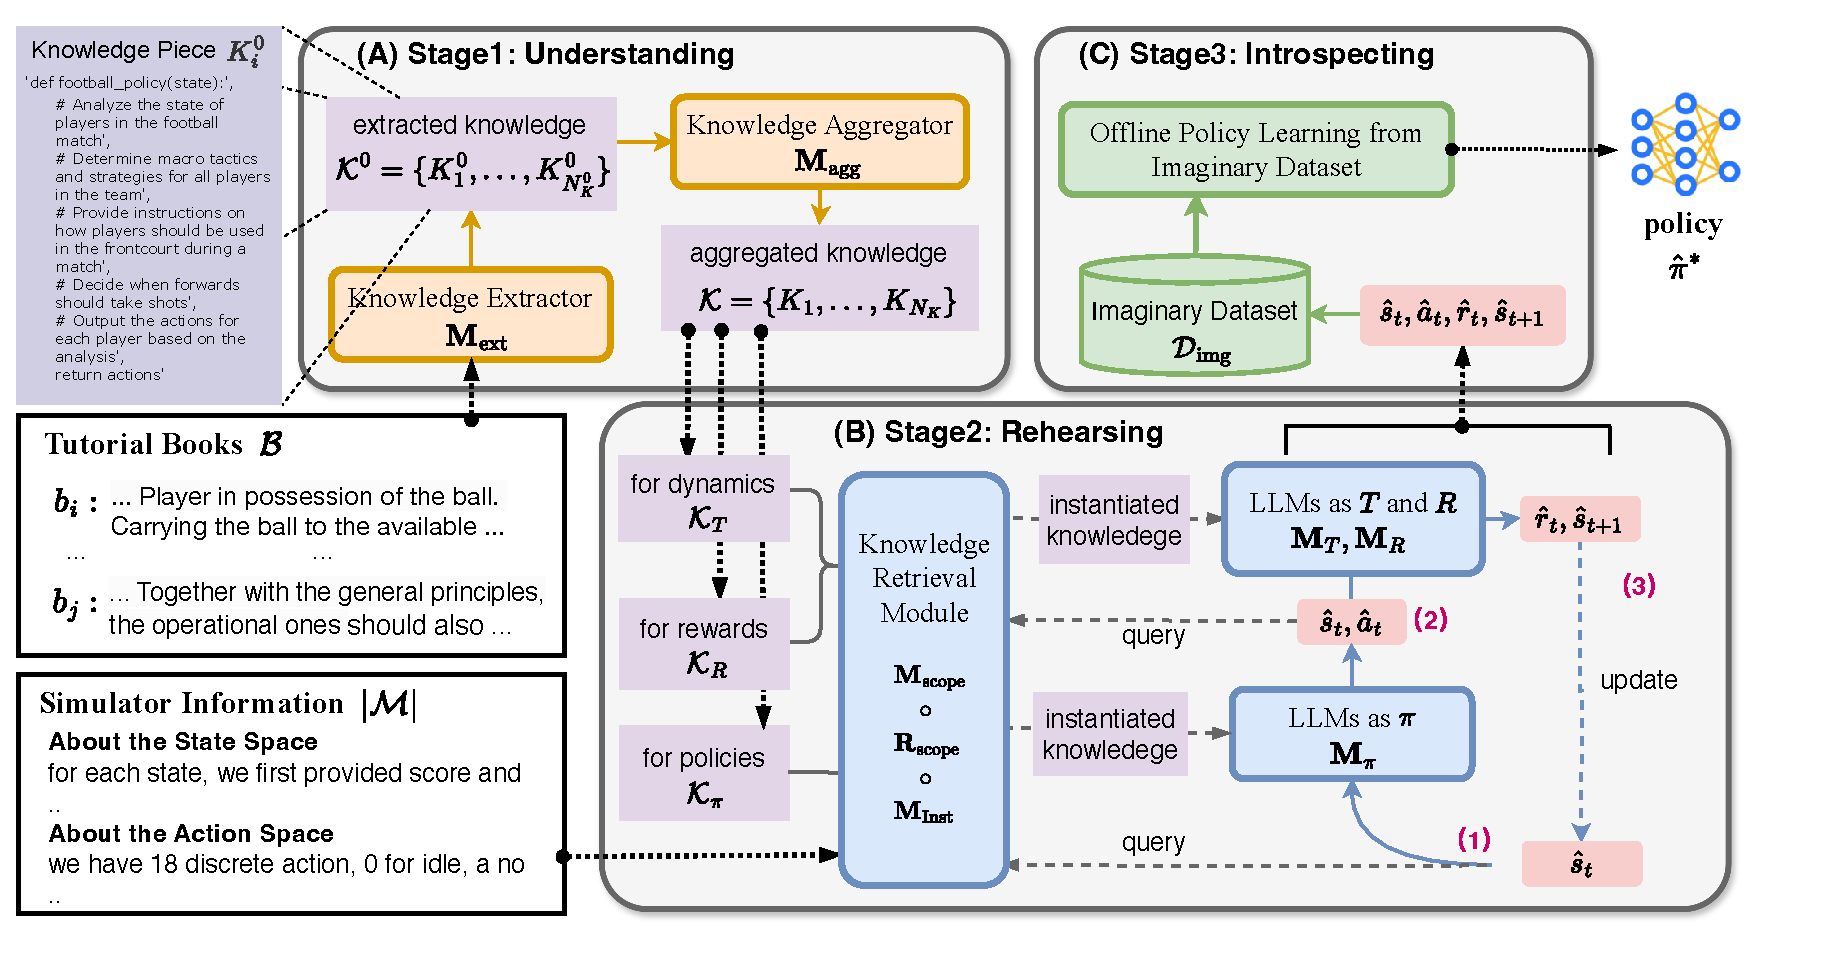
\includegraphics[width=1.06\linewidth]{fig/phrase-1.pdf}
    \vspace{-7mm}
    \caption{The URI pipeline consists of three major stages: (A) \textbf{Understanding:} The knowledge extractor and aggregator modules process paragraphs from books to form a structured knowledge database organized as pseudo-code. (B) \textbf{Rehearsing:} Using the knowledge database, the simulator generates and iterates through imagined states, actions, and rewards to create an extensive imaginary dataset. (C) \textbf{Introspecting:} The introspection module refines the policy network by evaluating and correcting errors in the generated states, actions, and rewards to ensure accurate and effective policy implementation.}
    \label{fig:3-stage-implmentation}
\vspace{-7mm}
\end{figure}

% \begin{figure}[t]
%     \vspace{-2em}
%     \centering
%     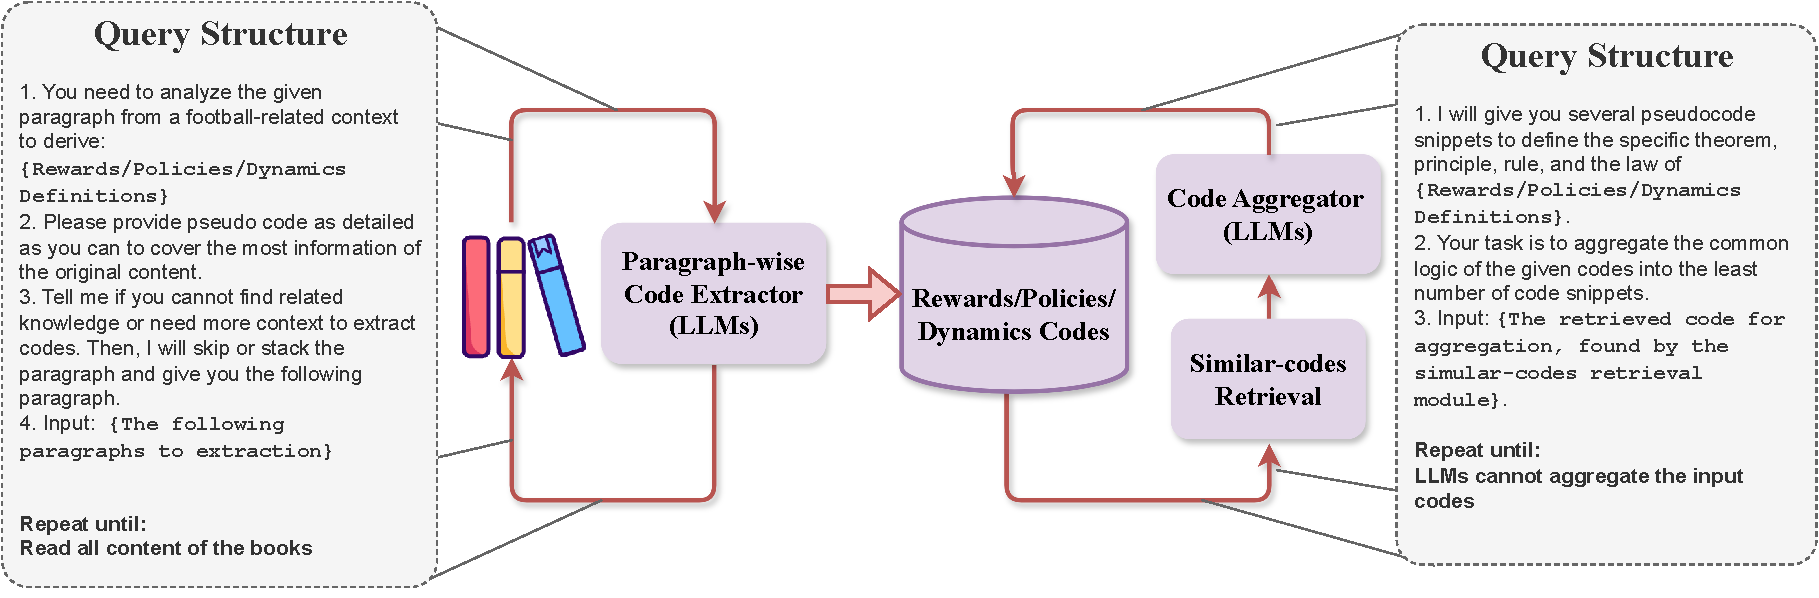
\includegraphics[width=0.2\linewidth]{fig/plb-understanding-v2 (2).pdf}
%     \caption{The procedure of understanding can be generally divided into paragraph-wise extraction (left) and iterative aggregation (right). Examples of the prompts of the two phases are also shown.  \cxh{TODO: polish this pic.}}
%     \label{fig:understanding}
% \end{figure}

% \begin{figure}[t]
%     \centering
%     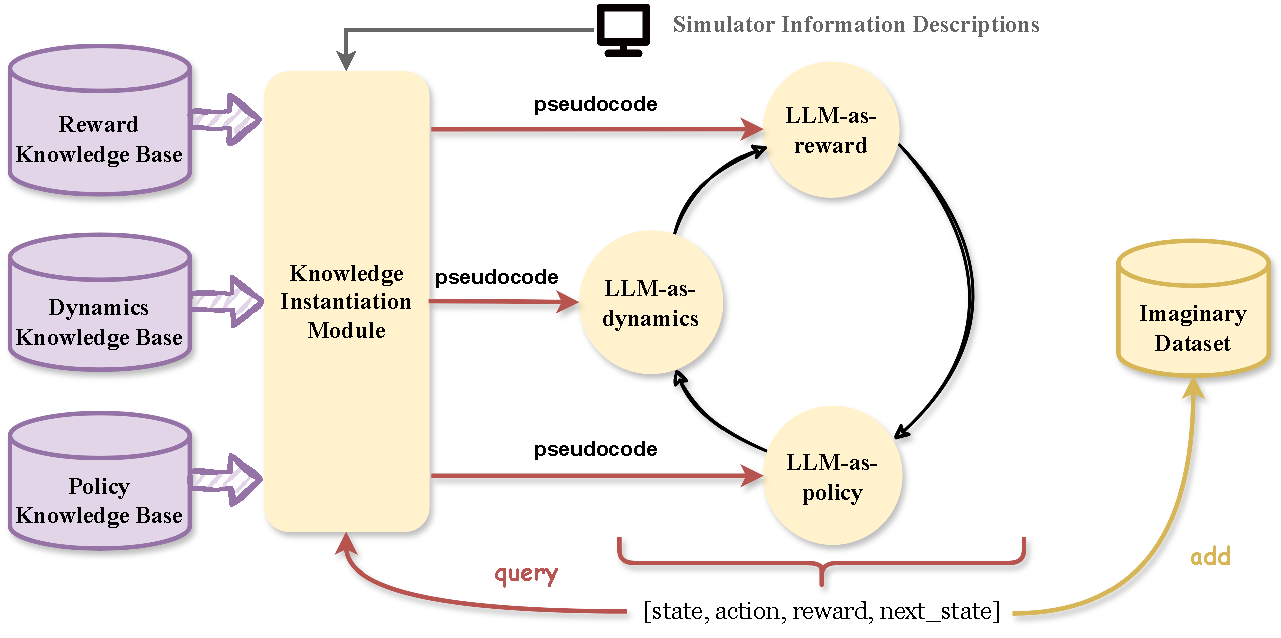
\includegraphics[width=0.2\linewidth]{fig/plfb-stage2-simp (4).pdf}
%     \caption{The procedure of retrieval relies on the code-based knowledge extracted in the understanding module (purple parts) to generate related policy, dynamics, and reward. All the generated data are stored in the imaginary dataset.
%     \yali{the figure is not clear to me. The query is given, but what's the output of this workflow? what is "simulator information description"?}}
%     \label{fig:retrieval}
% \vspace{-0.6cm}
% \end{figure}

The understanding module is responsible for extracting knowledge $\know:=\{K_1, ..., K_i, ..., K_{N_{K}}\}$ from the books $\books$, where $K_i$ denotes one piece of knowledge. For we humans, the knowledge is naturally stored in our brains. For machines, the first question is what should be the appropriate format to represent the knowledge. Since LLM has shown superior performance in code generation and codes themselves as interpretable, compact and expressive languages~\citep{llm-code2024ke}, we also choose it as the basic format of knowledge representation. Different from previous works~\citep{voyager2023guanzhi} which directly asked for runnable code for the downstream tasks using, we do not execute this code. Instead, we just use it as a more flexible and abstract description of the skill and transition while still maintaining a rigorous control flow.  As shown in Figure.~\ref{fig:3-stage-implmentation}(A), a knowledge extractor module is used as the first step. The knowledge extractor is an LLM-injected model. We iteratively ask $K_j=\llm_{\rm ext}(b_i)$ to examine whether a paragraph is related to the decision-making elements, i.e., policy functions, reward functions, dynamics functions, and how to represent them as pseudocode. 

% Books are usually long texts, possibly several hundred pages, and some of the contents are transitive words that are not directly related to skills, environment transition, and evaluations. 

Moreover, humans often learn by repeatedly reading the texts across pages and even books, by updating existing knowledge with newly learned ones and summarizing them into more general and abstract forms. A similar procedure is achieved by the knowledge aggregator module, shown in Figure.~\ref{fig:3-stage-implmentation}(A), as the second step of understanding. The knowledge aggregator is also an LLM-injected model. We iteratively ask $\llm_{\rm agg}([K_i, K_j, K_l, ...])$ to aggregate relevant knowledge among different segments based on a similarity estimation of the embedding model $\emb$. Formally, let $\know^0:=\{K_1^0, ..., K^0_{N_K^0}\}$ be the paragraph-wise knowledge extracted by $\llm_{\rm ext}$. For the $j$-the iteration, $[K^{j+1}_o, K^{j+1}_p, ...]=\llm_{\rm agg}([K^{j}_i, K^{j}_l, K^{j}_n, ...])$, where $[K^{j}_i, K^{j}_l, K^{j}_m, ...]$ is from $\know^j$ by selecting the most similar $N_{\rm agg}$ pieces of knowledge by comparing their cosine similarity under the embedding model $\emb(K)$ of GPT and $o,p,i,l,n$ here denote the indexes. $[K^{j+1}_o, K^{j+1}_p, ...]$ are then added to $\know^{j+1}$. 
% Formally, we denote the extract knowledge of the Knowledge Extractor
% The first step to understanding the contents is to identify where are the useful content, and 
% then an iterative aggregation of relevant paragraph-wise knowledge based on a similarity estimation will be adopted. 
The iteration will stop if $|\know^{j+1}|>=|\know^{j}|$, where $|\know^{j}|$ is the pieces of knowledge at $j$-th iteration. 
After iteration stops, the remaining knowledge pieces constitute the knowledge databases by splitting them into dynamics-related knowledge $\know_{\transf}$, reward-related knowledge $\know_{\rewf}$, and policy-related knowledge $\know_{\pi}$ for later modules to use. More details are provided in Appendix~\ref{app:understand}. 

% \cxh{We need A paragraph to summarize the output of the section.}
% Thanks to pseudo-codes themselves that they usually contain some descriptive words about their intent and algorithm, we use the embedding of them directly as its "key" for later retrieval rather than generating another separate annotation paragraph. 
% \textcolor{red}{We did not attempt to read the full book instantly since the summarizing done in this manner is less controllable, and the API is more expensive. }



% imaginary experience replay
\vspace{-1mm}
\subsection{Knowledge-based Rehearsing of Decision-Making}
\label{sec:rehearsing}
\vspace{-2mm}

% this section provides how we code -> data.
When humans develop a rough understanding of a new skill $\pi$ from knowledge $\know$, they will usually imagine what choice they will make given certain situations and what are the possible consequences in their minds. This rehearsing procedure would help humans correct apparent mistakes and consider better actions for long-term benefits~\citep{rehearsing@2024jia}. 


% Previous works, though encoding a search process in planning~\citep{tot2023shunyu, llm-mcts2023zirui}, or using multi-level planning to improve long-term LLM, still fail to form a closed-loop rehearsing without interaction with the environment. 
% While in \topic, we would like the LLM to generate not only the action but also the transition and the reward. 
% This full generation has two benefits: (1) it maximizes the use of knowledge in LLM acquired during the pre-training and extracted from the book; (2) it allows more flexibility in retrospecting the imagination. 
% The framework of \topic-retrieval is in Figure.~\ref{fig:retrieval}.
 
% \subsection{\mf{Imagined Data Generation}}
%{Imaginary Data Generation via Interactive Retrieval from Books}


We implement a closed-loop generation process involving the LLM-injected dynamics function $\llm_{\transf}$, reward function $\llm_{\rewf}$, and policy $\llm_{\pi}$, as depicted in Figure.~\ref{fig:3-stage-implmentation}(B). 
This approach resembles the model rollout in traditional model-based RL, where the policy, reward function, and dynamics function are represented by LLMs. Given the current imagined state $\hat s_t$, the LLMs $\llm_{\pi}$ first predict the most plausible action $\hat a_t$. Subsequently, $\llm_{\transf}$ and $\llm_{\rewf}$ generate the next state $\hat s_{t+1}$ and the associated reward $\hat r_{t}$ based on this action and the current state. In the process, a knowledge retrieval module is involved to select relevant knowledge pieces enhancing the LLM input with this information for LLM's predictions, e.g., $\hat a_{t}=\llm_{\pi}(\hat s_t, \ret(s_t, \know_{\pi}))$, $\hat r_t = \llm_{\rewf}(\hat s_t, \hat a_t, \ret(s_t, \know_{\rewf}))$ and $\hat s_{t+1} = \llm_{\transf}(\hat s_t, \hat a_t, \ret(s_t, \know_{\transf}))$. The knowledge retrieval module includes the following two steps:

\textbf{State-based Knowledge Scope Retrieval:}\label{sec:sbksr} 
% During data generation by LLMs, for each state, we initially retrieve the most relevant knowledge from our database, enhancing the LLM input with this information. 
% However, 
% Standard RAG techniques, i.e., embedding-vector similarity matching, do not work in this scenario. 
The fundamental problem of standard RAG techniques, i.e., embedding-vector similarity matching, in this scenario, is the modality gap between the query $s_t$ and the knowledge $\know$.
% Unlike standard RAG techniques, which rely on embedding-vector similarity matching, we confront a fundamental challenge due to the modality gap between the queries and the database contents. 
Standard RAG approaches aim to identify information closely related to the query, while here we need to ask the most suitable knowledge to be applied as a dynamics/reward/policy function \textit{that has the best predictions} for the queried state and action. Standard RAG techniques tend to retrieve knowledge pieces that include similar text patterns as the queried states and fail to find the best knowledge for predictions. To address this, we propose a knowledge scope retrieval method that includes a simple yet effective preprocessing step to bridge the modality gap. In particular, we traverse all knowledge pieces $K_i \in \know$ by iteratively sampling $n_{\rm scope}$ knowledge pieces $\{K_i\}_{n_{\rm scope}}$ from the database $\know$, combining them with simulator information $|\gM|$ and using LLM $\{K^S_i\}_{n_{\rm scope}}=\llm_{\rm scope}(\{K_i\}_{n_{\rm scope}},|\gM|)$ to determine the preferred scopes $K^S_i$ for each piece of knowledge. 
$K^S_i$ is defined by the preferred subspace of state to use the knowledge. Then a standard RAG technique is applied to identify the most relevant knowledge scope $K^s_j$ and its relevant knowledge $K_j$. Formally, $(\{K_j\}, \{K^S_j\})=\ret_{\rm scope}(\hat s, \know^{S})$, where $\know^{S}$ is the scopes of the knowledge database. This method is effective for embedding models in retrieving the correct knowledge as the texts of keys and queries both are about the descriptions of states. 
% one sentence summary about why  this work.

% concatenate with simulator information descriptions, e.g., the state space and action space of the football game simulator, ask LLMs for the preferred state scopes of each piece of sampled knowledge to serve as prior knowledge of rewards/dynamics/policy in the football game. Then, standard RAG techniques are applied by regarding the current state as the ``query'' and the preferred state scope as the ``key'' to find the relevant knowledge.


% When the LLMs generates data, for each state, we first need to retrieve the most relevant knowledge from the knowledge database and extend the input with the retrieved knowledge for LLMs. However, standard RAG techniques, i.e., embedding-vector similarity matching, do not work in this scenario. The fundamental problem is the modality gap between the query and the information in the database. The standard RAG techniques pursue finding the most relevant information between the query and the item in the database, while here we need to ask for the most suitable knowledge to be applied as a dynamics/reward/policy function in the queried state and action \textit{for the best predictions}. Standard RAG techniques will just tend to retrieve the knowledge that includes similar meanings as the queried states and fail to find the best knowledge for predictions. 

% In this article, we propose a simple yet effective retrieval method, which includes a prepossess step to bridge the modality gap. 
% In particular, we iterate choose $n_{\rm scope}$ pieces of code-based knowledge from the database, concatenate with simulator information descriptions, e.g., the state space and action space of the football game simulator, ask LLMs for the preferred state scopes of each piece of sampled knowledge to serve as prior knowledge of rewards/dynamics/policy in the football game. Then, standard RAG techniques are applied by regarding the current state as the ``query'' and the preferred state scope as the ``key'' to find the relevant knowledge.

\textbf{Post-Retrieval: Knowledge Instantiation:} Predicting based on code knowledge requires the LLM's robust understanding of code.  We refine this process employing an LLM to instantiate the code $K^I=\llm_{\rm Inst}(\hat s, |\mathcal{M}|, \{K_j\})$ based on the current state $\hat s$, the simulator information description $|\mathcal{M}|$ and the knowledge $\{K_j\}$ retrieved by $\ret_{\rm scope}$.
Knowledge instantiation involves generating a specific pseudocode based on the football-related knowledge coded in the retrieved information, tailored to the simulator's current state and action requirements. 
% In this way, the instantiated pseudocode conforms to the simulator's design, suggesting actions, rewards, or subsequent states based on the observed information. 

Finally, three LLMs are involved to generate the imaginary dataset $\mathcal{D}_{\rm img}$, including $\hat a_{t}=\llm_{\pi}(\hat s_t, \llm_{\rm Inst}(s_t, |\mathcal{M}|, \ret_{\rm scope}({\hat s}, \know_{\pi}^S)))$, $\hat r_{t}=\llm_{\rewf}(\hat s_t, \hat a_t, \llm_{\rm Inst}(s_t, |\mathcal{M}|, \ret_{\rm scope}({\hat s}, \know_{\rewf}^S)))$ and~$\hat s_{t+1}=\llm_{\transf}(\hat s_t, \hat a_{t}, \llm_{\rm Inst}(s_t, |\mathcal{M}|, \ret_{\rm scope}({\hat s}, \know_{\transf}^S)))$, where $\know_{\pi}^S$, $\know_{\rewf}^S$, and $\know_{\transf}^S$ are the scope of the knowledge database $\know_{\pi}$, $\know_{\rewf}$, and $\know_{\transf}$ respectively. To start the rollout of a trajectory, we need a state as the initial state. It has several choices to achieve, e.g., sampled from $\gS$, generated by another LLM, or pre-collected a small number of real states from the target environments as part of simulator information. Since the first two choices might involve more unrealistic initial states, to simplify the difficulty of the task, we pre-collected a small number of real states in this article. The detailed setup is in the experiment section. Besides, during the rollout over $H$ steps, we reuse instantiated knowledge to reduce the overload of LLM's callings. More details are provided in Appendix~\ref{app:rehearsing}.
% This approach offers two advantages: it reduces the number of calls to the more powerful LLM, thus lowering calling costs, and it explicitly translates general football knowledge into specific knowledge relevant to the current simulator state, enhancing the LLM's effectiveness in downstream tasks. 
  
% 基于代码知识做出对应的决策需要依赖于更大规模的LLMs,实现对代码的强理解。而大的语言模型(比如GPT4)意味着较高的调用成本。为了生成大量数据,我们需要反复的调用LLM,这意味着较大的成本开销。本文对这个问题做了一个优化。具体而言,我们使用较强的LLM (GPT-4) 来根据当前的状态,动作信息,simulator information description,和Retrieved Knowledge实例化代码。实例化指的是,根据retrieved得到的基于代码表示的对于football本身的knowledge,根据当前的simulator的information,和具体面临的state和action给出更具体的伪代码,他根据状态空间提供的观测信息给出符合模拟器设计规范的对应的动作,奖励值,或者下一步的状态。之后,在rollout的$n_{\rm repest}$步过程中,我们会复用这个实例化的代码,使用较弱的语言模型来实现reward,dynamics和policy的功能。这么做有两个好处,(1)减小了调用了强语言模型的次数,降低了开销;(2)实例化的过程中把general的football相关的knowledge transfer成了根据当前的simulator和具体面临的state相关的具体的knowledge。

% adopt the retrieval-augmented generation technique. When the LLM generates the data, it first retrieves the most relevant knowledge from the database collected in the previous stage and extends the input with the retrieved knowledge. The relevance is measured by the embedding lookup based on the current state. A two-level generation implements the rehearsing. The higher level is responsible for outputting general and long-term instructions about the game whose inputs are merely the current state. The lower level, given the strategy generated by the higher level, is specialized to output environment-related actions. This two-level generation also promotes the reuse of the general knowledge across tasks of a similar field: only the low-level environment-specific generation needs to adapt.



% \begin{figure*}
%     \centering
%     \includegraphics[width=0.95\linewidth]{fig/per-retrieval.pdf}
%     \caption{Illustration of the book-retrieval module and the imaginary data generator.}
%     \label{fig:retrieval}
% \end{figure*}


% \sy{some prompt and output example}
\vspace{-5mm}
\subsection{Introspecting based on the Imaginary Dataset}
\label{sec:introspecting}
\vspace{-2mm}

% \textbf{Offline RL} addresses the problem of learning policies from a pre-collected dataset~\citep{cql@2020aviral,dsconstraint@2023ran,mopo@2020tianhe,maple@2023xionghui, mobile@sun2023}. 
% Existing works can be classified into two categories: model-free and model-based methods. Model-free~\citep{brac@2019yifan, td3-bc@2021fujimoto, bear@aviral2019, rem@2020rishabh, cql@2020aviral, iql@2021kostrikov, dsconstraint@2023ran} methods learn a conservative policy directly from the dataset. 
% Model-based offline algorithms~\citep{mopo@2020tianhe, morel@2022rahul, maple@2023xionghui, mobile@sun2023, genoffline@luo2024} first estimate a model from the dataset and perform policy learning or planning based on this learned model. 
% In our work, to achieve introspection from data generated by LLMs, we build our policy distillation algorithm based on several existing techniques in offline RL, including the uncertainty penalty in Model-based Offline Policy Optimization (MOPO)~\citep{mopo@2020tianhe}, which constructs a pessimistic model that discourages the policy from visiting states where the model is inaccurate; and a model-free method, Conservative Q-learning~\citep{cql@2020aviral} to obtain a robust value function that does not overestimate unseen state-action pairs too much.

% What is X for human beings?
% What is the purpose of X in \topic?
% What is the challenge of implementing X?
% how do we handle these challenges?
% \cxh{Maybe we can follow : (1) What is X for human beings? (2)  What is the purpose of X in \topic?; (3) What is the challenge of implementing X?; (4) how do we handle these challenges? for these three subsection.}
The direct output LLM in the rehearsing stage can be sub-optimal or incorrect. We would like to re-examine the collected data and try to distill a policy that can avoid the side effects. 
% This distillation also brings practical benefits: only the small policy, instead of the LLM, is needed for the final deployment which drastically reduces the deployment cost. 
We can regard the data $\mathcal{D}_{\rm img}$ collected during the rehearsing stage as an offline dataset and apply offline RL algorithms to train an improved policy from the dataset. 
However, directly applying existing offline RL algorithms over-simplifies the problem. Compared with the standard offline setting where only the behavior policy is sub-optimal, there is an additional misalignment in the data generated during the rehearsal: the transition and the reward function estimated by the LLM are also inaccurate. Overlooking such inaccuracy would result in a policy exploiting the sub-optimal transition and reward function and cause performance degradation or even risky behaviors in the final deployment. 

To solve the problem, in this paper, we adopt the Conservative Q-learning ~\citep{cql@2020aviral} as the base offline RL algorithm, whose learning objective is as follows:
\begin{small}
$$\begin{aligned}
\min _Q \max_\pi~&\alpha\left(\mathbb{E}_{\hat s \sim \mathcal{D}_{\rm img}, a \sim \pi(a \mid \hat s)}\left[Q(\hat s, a)\right]-\mathbb{E}_{\hat s, \hat a \sim \mathcal{D}_{\rm img}}[Q(\hat s, \hat a)]+\mathcal{R}(\pi)\right)  +\mathbb{E}_{\hat s, \hat a \sim \mathcal{D}_{\rm img}}[(Q(\hat s, \hat a)-\hat{\mathcal{B}}^{\pi} \hat{Q}(\hat s, \hat a))^2],
\end{aligned}$$
\end{small}
where $\hat{\mathcal{B}}^{\pi} \hat{Q}$ is the bellman update operator to update the Q-value function~\citep{rl@2018sutton}, and the first term is to learn a policy with conservative Q value~\citep{cql@2020aviral}. As a solution of introspecting from imaginary data, as shown in Figure.~\ref{fig:3-stage-implmentation}(C), we add the uncertainty of the reward and transition estimation as the regularization terms, $\mathcal{R}_{\rewf}$ and $\mathcal{R}_{\transf}$ over the original reward $\hat r$ output by the LLM $\llm_{\rewf}$. In practice, we adopt these regularization terms by applying them when we backup the $\hat Q^k$:
\begin{align*}
    \hat{\mathcal{B}}^{\pi}_{\rm I} \hat{Q}(\hat s, \hat a) := \hat r - \eta_{\rewf} \mathcal{R}_{\rewf}(\hat s, \hat a) - \eta_{\transf} \mathcal{R}_{\transf}(\hat s, \hat a) + \gamma \mathbb{E}_{\hat s' \sim \mathcal{D}_{\rm img}, a' \sim \pi_k(a' |\hat s')}[Q(\hat s', a') ],
\end{align*}
where $\hat s' \sim \mathcal{D}_{\rm img}$ is to sample the next state given $\hat s, \hat a$, $\eta_\rewf$ and $\eta_\transf$ are two hyper-parameters to control the weighting of the uncertainty terms. Inspired by Model-based Offline Policy Optimization (MOPO)~\citep{mopo@2020tianhe}, the uncertainty is estimated by an ensemble of $N_{\rm ens}$ Gaussian models of $\hat \transf$ and $\hat \rewf$, which is learned by maximizing logarithmic likelihood from the imaginary dataset. Then the uncertainty is estimated by $\mathcal{R}_{\rewf}(s, a) = \max_{i\in\{1, \dots, N_{\rm ens}\}} \sigma^r_i(s, a)$ and $\mathcal{R}_{\transf}(s, a)=\max_{i\in\{1, \dots, N_{\rm ens}\}} \sigma^T_i(s, a)$, where $\sigma^r_i$ and $\sigma^T_i$ are the $i$-th reward and dynamics model's predicted standard deviation for $s, a$ respectively. We call the solution of CQL with $\hat{\mathcal{B}}^{\pi}_{\rm I}$ as the bellman update operator Conservative Imaginary Q-Learning (CIQL). 
This regularization is easy to implement and can force the policy to generalize better over the regions where the LLM outputs inconsistent next states and rewards.